\section{Method}\label{method}
As described in the introduction the ability to detect the hand of the robot, 
firstly presupposes the localization of regions that show alike and causal 
movement within the scene. For that we start by tracking all possible flocks 
of candidate regions in the image. Candidate regions are image patches of 
size $N \times N$ pixels that can be tracked well and where its containing 
features define a clear and unambiguous common direction. Concurrently to 
the tracking, the relative motion of the arm joints is recorded in order 
to have a base for comparing the visual information in the decisive step 
where all the visually gained trajectories are correlated with the arm joint. 

% ***********************************************************************************************
The ability to subsequently detect the hand of the robot, firstly presupposes the localization of regions that show alike and causal movement within the scene, as already introduced in section \ref{intro}. For that we start by tracking all possible flocks of candidate regions in order to determine which of the moving regions could be a part of the robot. Candidate regions are image patches of size $N \times N$ pixels that can be tracked well and where its containing features define a clear and unambiguous common direction. Concurrently to the tracking, the relative motion of the moving arm joint is recorded in order to have a base for comparing the visual information in the decisive step where all the visually gained trajectories are correlated with the single arm joint behaviour. 
%
%

% -----------------------------------------------------------------------------------------------
%
%																			localization - Assumptions
%
\subsection{Assumptions}\label{method:localization:assumptions}
% -----------------------------------------------------------------------------------------------

Proprioceptive feedback allows us a lot of information to exploit for various 
tasks. As soon as James generates motion with its arm as sort of 
self-exploratory motion generation it will cause changes in the visual and 
sensory perception. The robot senses a moving arm part which again indicates 
him to be attentive on visual feedback. \textit{Feeling} changes, means that 
there is the possibility to \textit{see} some changes which will then be 
correlated to the self-caused action behavior. At the current stage of 
development of this algorithm a few assumptions have to be set. The single 
arm joint motion

\begin{enumerate}
	\item produces enough net displacement in the plane parallel to the camera's CCD,
	\item takes place within the visual field of the robot's eye
	\item while James is neither moving its head nor its eye.
\end{enumerate}
In later stages of these works maybe all these constraints can be eliminated or at least incrementally eliminated.

Moving several joints at the same time or also moving different joints consecutively produces a complex movement in space (3D). This algorithm, however, is not yet using stereo vision. As a consequence of the missing dimension and the inexistence of a kinematic model of the arm (and rest of the body) it is not possible to calculate spatial motion out of two dimensional visual data. So, periodical waving or randomly moving one arm joint must mainly effect enough net displacement in a 2D plane parallel to the eyes' CCD element. 
To ensure this constraint an omnipotent criteria $ C_t $ is introduced that allows to move one single joint only, over an appropriate time interval. Looking back in the past at each time step using the standard deviation of the differences, ensures to transport the constraint over the whole interval, with a "safe" and short interrupt window.  In case of violation the algorithm starts newly or in an advanced stadium tries to localize the hand from the so far gathered information. We use the standard deviation to forgive the joints a possible change of the encoder values due to a shaking movement of another body part or joint. A shudder eventually causes a small peak in the time-elongation diagram of a joint $k$ that is thus robustly cushioned and not detected as intentional actuation.
%
We do not always receive stabilized images, even if the neck, head and eye actuators did not perform any active motion or somebody does walk somewhere through the scene, what in both cases could be understood as visible motion of the arm. Therefore the motion in the image has to exceed a certain motion threshold that is dependent on the focal of the eye's lens.
%
% -----------------------------------------------------------------------------------------------
%
%																						localization
%
\subsection{Localization}\label{method:localization}
% -----------------------------------------------------------------------------------------------
According to the approach, the attention system waits for a significant visual change in the scene. Due to the robot's ignorance of understanding the scene, any motion will be considered important that is greater than a certain amount. For a human being it is easy to make out and distinguish coherent and relevant regions. The following steps propose a possibility for the robot to do so as well.\\ \newline
%
% -----------------------------------------------------------------------------------------------
%
%\subsubsection{Classification of the optical flow}\label{method:localization:classification}
%\textbf{1) Classification of the optical flow}\newline%\label{method:localization:classification}
\textit{1) Classification of the optical flow}\\ \newline
% -----------------------------------------------------------------------------------------------
In order to localize regions that belong together, in sense of motion, we must first classify these regions and segment the global motion in the scene. Smaller regions that move together \textbf{within a larger neighbourhood } will later be put together into unique identifiable patches that contain several neighboured locations in the image moving equally and in the same direction.\\ \newline
%
% -----------------------------------------------------------------------------------------------
% 1
\textit{1.1: Motion computation}\\ \newline
% -----------------------------------------------------------------------------------------------
Between two consecutive time frames the motion is computed in a classical way where motion is computed by first selecting traceable points in the scene and then the displacement is calculated.
\begin{enumerate}
	\item \textit{Feature selection: } We pick a high number of good features, e.g.\ $n=1000$, to track and calculate for the selected number \textit{n} of features their position in the next image with the following step. A feature selection that is \textit{optimal by construction} for which tracking produces good results %not only for translational but also for affine motion 
	is the one proposed by J. Shi et. al\ \cite{GFT94-06}. %Using this technique assures a reliable choice for each type of motion.
	\item \textit{Feature tracking :} The pyramidal Lucas Kanade feature tracker searches in the image $I_t$ all features that were previously found \cite{PILKFT99} %. The Lukas Kanade tracker 
	and can be seen as a function that returns for each given feature in image $I_{t-1}$ the location in $I_{t}$ and receive $n$ displacement vectors; information that is describing the behaviour of the scene in the image.%\\ \newline
\end{enumerate}
%
% -----------------------------------------------------------------------------------------------
% 2
\textit{1.2: Patching the flow} \\ \newline
% -----------------------------------------------------------------------------------------------
As long as step 1.4 is unmet, the image is divided into a grid (step 1.2a)\ ) of equilateral patches where each optical flow is inserted and we start the classification process of the optic flow and decide on the regions belonging together. An object wandering through a scene projects in the image plane an area with an equivalent motion, thus this region is likely to own many optical flow vectors with similar or even equal values pointing to the same direction. Dividing the object's projection in the image plane into image patches must also divide the flow vectors into patches. These, into patches, summarized features are subregions that must still be moving like the corresponding object. \newline
On the other hand, if patches have already been initialized, the optical flow is placed in its corresponding patch (step 1.2b)\ ). \newline
%
% -----------------------------------------------------------------------------------------------
% 2a
%\paragraph{Step 3a): Initialization of the patches}\label{method:localization:classification:step3a}
\textit{a): Abstraction, initialization of the patches} \newline
% -----------------------------------------------------------------------------------------------
The result from the upper step 1), the current image, is first divided into a grid with $n_w \times n_h$ 2D patches where $n_w = \lfloor \frac{w}{N} \rfloor$, analogous for the height $n_h$, because $\vert \Lambda \vert = N \times N$ and the image size: $\vert I_{x,y} \vert = w \times h$. \newline
%Grid cells that eventually do not span the size of an ordinary patch are generously omitted, what means a maximal loss of the last $w \times (N-1)$ pixels in the height and the last $h \times (N-1)$ pixels in the width. Overall it does not make a big difference about the information content of the image. 
%Every patch $\Lambda_{F_k}$ covers in the initialization image cell \textit{i}, where the center of the patch \textit{(i,j)} is defined by:
%\begin{equation}
%\label{centering}
%center\left( \Lambda_{F_k} \right) =  \vec{c}_k\left( i, j \right) = \begin{pmatrix}i*N  + \frac{N}{2} \\ j*N  + \frac{N}{2}  \end{pmatrix}, \quad \forall i = 0 \ldots n_w \mbox{ and } \forall j=0\ldots n_h  \enspace .
%\end{equation}
%
% -----------------------------------------------------------------------------------------------
% 2b
%\paragraph{Step 3b): Assigning features (patching the flow):}\label{method:localization:classification:step3b}
\textit{b) Assigning features' flow to its patch} \newline
% -----------------------------------------------------------------------------------------------
Each feature is dropped into the cell according to its position. Consequently a patch $\Lambda_{F_k}$ absorbs all the displacement vectors that lie in the fixed patch size at the current position.\\
%:
%\begin{equation}
%\forall k = 1\ldots n: \quad center \left( \vec{d}_k \right)  =  center \left( \Lambda_{F_i}  \right),  \quad \mbox{where } \vec{u}_k \in \begin{bmatrix} c_x \pm \frac{N}{2} \\ c_y \pm \frac{N}{2} \end{bmatrix} \enspace .
%\end{equation}
%%
\begin{figure}
	\begin{center}
		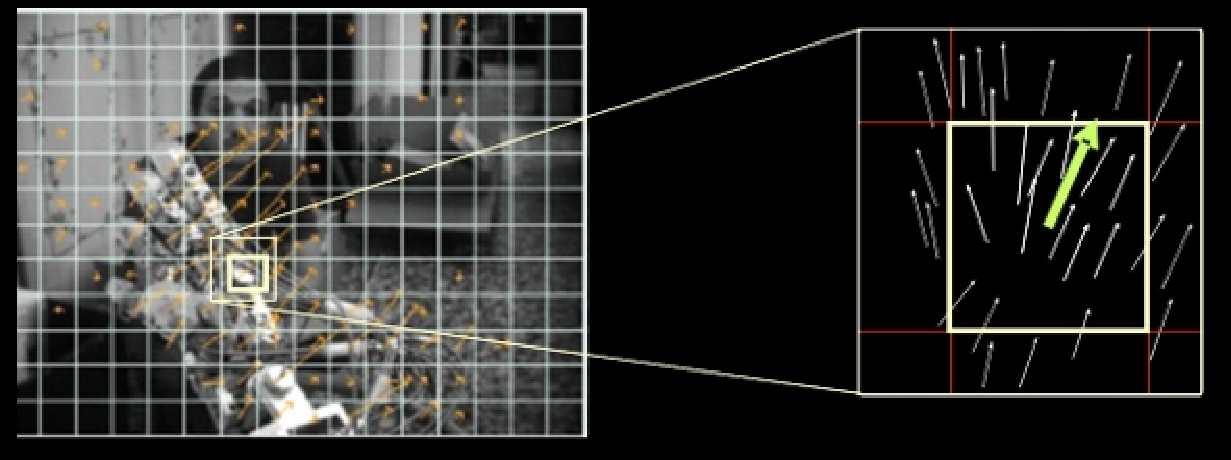
\includegraphics[width=3in]{imgs/method/step1to4.ps}
		\caption[Patching the flow. ]{\textbf{\textit{Patching the flow. Top left schematically shows an image extract with feature points and their displacements. As long as step 5 is not yet fulfilled, the image is subdivided into a grid of patches (top middle). Each cell in the grid assimilates all optical flow that is situated on its area (top right), however, if step 5 was satisfied and the tracking process is afoot, only relevant patches assimilate optical flow from newly determined features. The lower row illustrates step 4. }}}
		\label{fig:abstraction}
	\end{center}
\end{figure}
%
With this step the most important abstraction in the localization and detection process has been performed. Locations in the image array are decoupled from their original domain, the grey-level values (consult figure \ref{fig:abstraction} for the abstraction process). Our new informative system is a grid structure where each cell contains the correspondent set of displacement vectors $ \vec{d_i} \in \Lambda_k $ which are all centralized to the cell's center in respect to their start point. A set of loose values is not really classifying a small $ N \times N $ regions, much less larger regions. Likewise completely different displacement directions and amounts fall into the same $ \Lambda $ because the grid is placed over the image in a fix way, regardless the relationships in the scene.\\ \newline
%
% -----------------------------------------------------------------------------------------------
% 3
\textit{1.3: Representative patch displacement} \\ \newline
% -----------------------------------------------------------------------------------------------
After inserting all vectors in the patched image, for each patch the representative displacement is calculated. Each patch that has more than a certain amount of vectors greater than zero (that means traceable motion) are taken into account.
\begin{enumerate}
	\item \textit{Average angle}: In order to discard outliers in noisy regions and to tell the effective main direction of the patch, the angles must pass a corresponding confidence interval of the normal standard deviation of its comembers' values.
	\item \textit{General displacement vector}: Building the resultant (adding up the components) of the selected vectors leads to the common direction displacement of the patch.
\end{enumerate}
%
A reliable feature to classify the motion properties of the tracked image locations yields the direction component without building dependencies among the different $ \vec{v}_k = \vec{u}_k + \vec{d}_k $. Considering direction plus the velocity were building a strong unfoldable dependency for detecting these large regions. Apart from this fact, features sticking tight on a region that is spanning many patches, means an equivalent speed. So the velocity only differs in patches that lie on boarder regions of the object where there is anyway existing noise. The amount of the velocity is in neither of both directional classification cases an information with a qualitative statement, however, for the average displacement it matters. Additionally, due to the ratio between image size and patch size, where a single patch makes out at most approximately one per cent\footnote{In our set up $ percentage \left(  \Lambda, I \right) = \frac{N^2}{w*h}$ , where images have size 320 by 240 and $n < 20$ } of the whole image, the $ \vec{d}_k $ are assumed to be independently distributed  (in respect to their angle) at this point of time. We use the Gaussian distribution in order to determine a 90-percent confidence interval on the standard deviation of the angular values respective to the average angle of all $\vec{d}_k $ to eliminate the gross outliers. In figure \ref{fig:abstraction} we schematically sketched the representative displacement vector $\overline{\vec{d}_k}$ of patch $k$. Let us denote a set $\mathcal{A}$ that accommodates all $\vec{d}_i \in \Lambda_k$ that pass the 90-percent interval.% in equation \ref{confint}. 
Noisy regions are likely to be disqualified already here, otherwise at the next steps. Patches without any displacement logically go into the discard. 
%\begin{equation}
%	\alpha_{d_i} = \arctan{ \left( \frac{d_{i,y} }{d_{i,x} } \right)}, \quad \mbox{where } \forall \vec{d}_i \in \Lambda_{k} , i=0 \ldots n_{d_k} \enspace .
%\end{equation} 
%\begin{equation}
%\label{alg:avg}
%\overline{\alpha}_{d_k} = \overline{ \alpha } \left( \Lambda_k \right)  = \frac{1}{n_{d_k}} \sum_{i=0}^{n_{d_k}-1} \alpha_{d_i} \enspace .
%\end{equation}
%%
%\begin{equation}
%\label{alg:std}
%\sigma_{d_k} \approx \sqrt{ \frac{1}{n_{d_k} - 1} \sum_{d_i \in \Lambda_k} \left[ \left( \alpha_{d_i} - \overline{ \alpha}_{d_k} \right) ^2\right] } \enspace .
%\end{equation}
%
%Building the average and standard deviation on :
%
By first building the average and the standard deviation on the the angles $\alpha_{d_i}$, the 90-percent confidence interval and its $t$ as the $95^{th}$ percentile of the Gaussian distribution, where $\Pr\left(-t<A<t\right)=0.9$, can be defined as:
%
\begin{equation}
\label{confint}
\begin{bmatrix}  \overline{ \alpha}_{d_i} - \dfrac{t*\sigma_{d_k}}{\sqrt {n_{d_k}} } \end{bmatrix} 
\leq \alpha_{d_i} \leq 
\begin{bmatrix} \overline{ \alpha}_{d_i} + \dfrac{t*\sigma_{d_k}}{\sqrt {n_{d_k}} } \end{bmatrix} \enspace .
\end{equation}
%
Finally all $|\mathcal{A}|$ displacement vectors whose angles passed the 90-percent interval are building a resultant that depicts the representative displacement for that patch:
%
\begin{equation}
\label{representative}
\overline{ \vec{d_k }} =  \sum_{j \in \mathcal{A}}{\frac{\vec{d}_j}{|\mathcal{A}|} } \enspace .
\end{equation}
\\ \newline
%
% -----------------------------------------------------------------------------------------------
% 4
\textit{1.4: Clustering the patches} \\ \newline
% -----------------------------------------------------------------------------------------------
As long as this step did not succeed in a satisfying manner or is performed the first time the following classification step must be executed. For each patch $i$ with an angular value its eight neighbours are inspected to decide if the patch shall be marked for tracking. 
\begin{figure}
	\begin{center}
		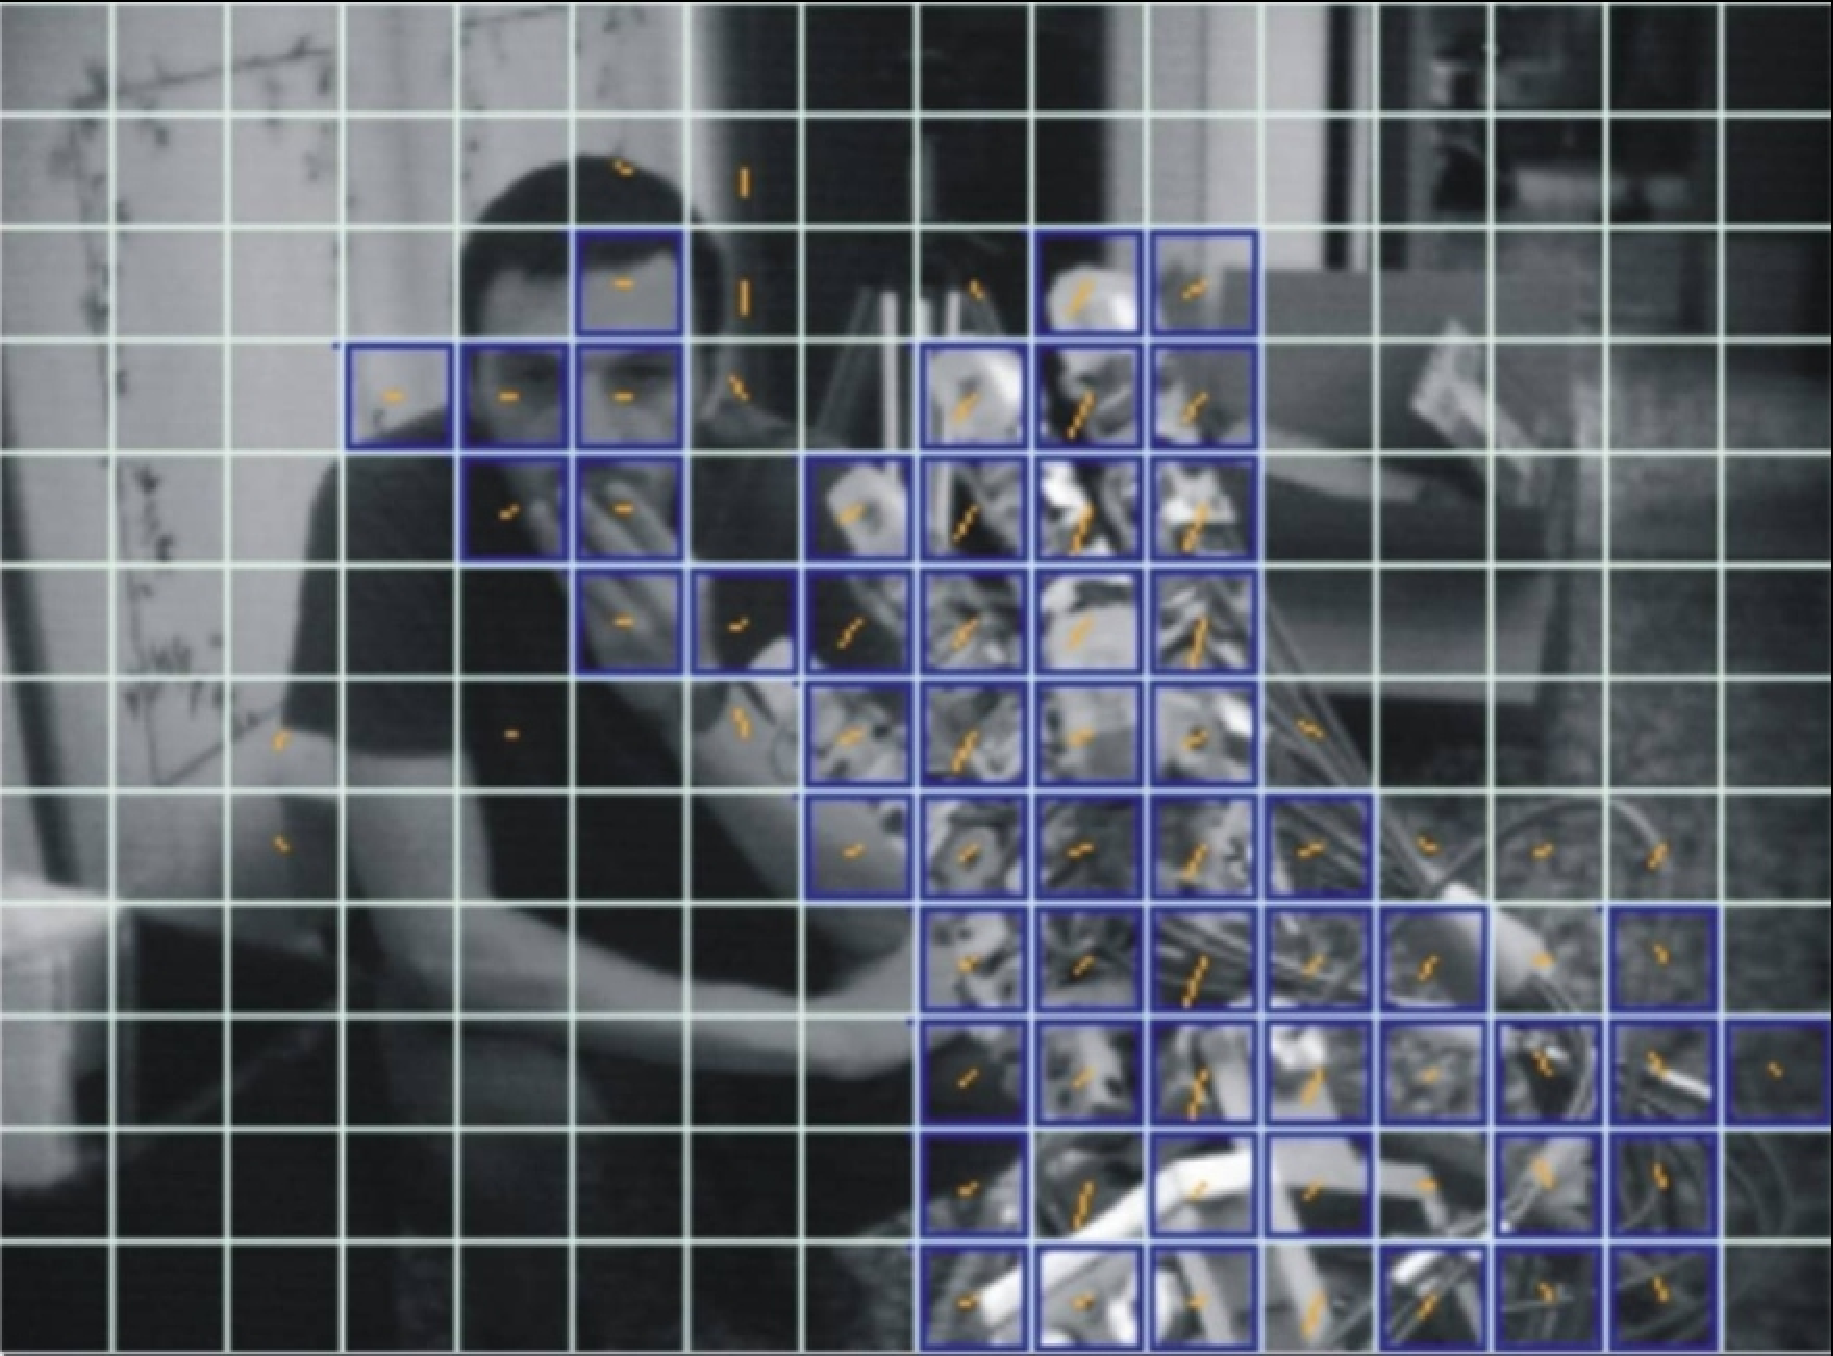
\includegraphics[width=2in]{imgs/method/selection.ps}
		\caption[Feature patch grouping. ]{Feature patch grouping. For each patch in the grid the neighbours are contemplated. If a patch has more neighbours than a minimal threshold $\rho_{MIN\_NEIGHBOURS}$ fulfilling that their direction in motion is lying between $\pm \beta_{range}$, it is marked as a relevant patch. As this process continues in the end we have flocks of patches that cover a bigger region moving in the same way, what can be seen as visual grouping according to \cite{ULGII23} }
		\label{fig:flocking}
	\end{center}
\end{figure}
%
A new threshold $\rho_{flow}$ ensures that not single patches or too small areas will be tracked, thus one single patch, e.g.\ with the size of $13 \times 13$, with no neighbour-patches is unlikely to depict a ``bigger'' region. A perfect coverage of the whole objects would be nice, but hardly possible to achieve. Reasons are the limited amount of features that are not equivalently distributed over all moving object, or that an object's surface is simply not have enough well traceable features. The aggregation of single patches to larger and distinct flocks of patches with "equidirectionally" motion among each other %is likely to happen 
turns up the for different objects with different motion trajectories. Coherent patches show a sufficiently equivalent direction compared to its neighbour according to a predefined aperture angle window. All patches that have more than a number of directly adjacent patches with the same behaviour, e.g. two out of an 8-neighbourhood in our setup, satisfying  $\beta_{range}$ get an unique identity and are kept for tracking.
% The just performed flocking of patches, again, does not necessarily cover a single object, but all the moving objects satisfying the above qualifications.	So, technically speaking for every patch $i$ with an angular value its eight neighbours are inspected to decide if the patch will be marked for tracking, see illustration in figure \ref{fig:flocking}. This importance measure is calculated by visiting all 8 neighbours according to the following scheme: \\
If the patch has a neighbour lying within an angular range (e.g +/-25 degrees) of the start patch's average angle, the neighbour patch is assumed to belong to the same region and therefore increases the importance measure of patch $i$ (see equation \ref{neighbours}). One patch can have at most eight neighbours pointing to the same direction. \\
%As we visit each grid cell on the patch image and determine the importance for tracking this cell we discard regions that remain alone or are not interesting to track. Obviously several flocks of patches with different values can be passed for tracking; where as each flock denotes a huge set of pixels that are very likely to move \textit{together} and belong to any moving object in the image fulfilling all conditions till this point.
%%
%\begin{equation}
%\label{neighbours}
%	neighbours\left( \Lambda_k\right) \ = \sum_{j=1}^{8} \omega_{kj}, 
%	\quad \mbox{ where } \omega_{kj} = 
%	\begin{cases}
%		1, & \mbox{if } 
%			\vert \overline{\alpha}_k  - \overline{\alpha} \left( neighbour \left( \Lambda_k, j \right) \right) \vert \leq \beta_{range} \\ 
%		0, & \mbox{else. } 
%	\end{cases}
%\enspace .
%\end{equation}
%The set $Q$ of patches that get qualified, due to their neighbour-relationships, is defined by:
%\begin{equation}
%\label{qualify}
%	Q\ = \left\lbrace \left( \Lambda_k \right): neighbours\left( \Lambda_k\right)  \geq \rho_{MIN\_NEIGHBOURS} \right\rbrace \enspace .
%\end{equation}
%In other words, the set of all patches (the entire image) will be divided in two disjoint sets such that: $I \left( t\right) = Q \cup \overline{Q}$ and $Q \cap \overline{Q} = \emptyset$.
%%
%Similar to the previous step, where the overall motion in the image must be higher than threshold $\rho_{motion}$, the overall percentage of selected patches must exceed $\rho_{flow}$ so that condition 
%\[
%C3: \quad \dfrac{\vert Q \vert}{\vert Q \vert + \vert \overline{Q} \vert} > \rho_{flow} \enspace .
%\]
%%
In other words, the set of all patches (the entire image) will be divided in two disjoint sets such that: $I \left( t\right) = Q \cup \overline{Q}$ and $Q \cap \overline{Q} = \emptyset$.
As long as this threshold is not fulfilled the whole procedure `%(all steps of 2)
 is continuously repeated. The example in figure \ref{fig:classified} shows the flocked regions, the head and the robot's hand. 
%
%\begin{figure}[H]
%	\begin{center}
%		\includegraphics[width=.90\textwidth]{data/images/halo/classified.jpg}
%		\caption[Grouped features worth to track. ]{Grouped features worth to track. Two images of a sequence that show in what fulfilling all conditions until step 3 result into; on the left hand side the binarized image difference from I(t) and I(t-1) and their optical flow }
%		\label{fig:classified}
%	\end{center}
%\end{figure}
%
\\ \newline
%
% -----------------------------------------------------------------------------------------------
%
\textit{2) Tracking and Correlation}\\ \newline
% -----------------------------------------------------------------------------------------------
% 2
By the time the classification provides one or several flocks marked as important regions in the scene, the tracking process launches.% At each point in time the displacement of each identifiable patch is recorded, where steps 1 to 4 supply the tracker with the needed information. 
%But as we later want to close the action-perception loop, we also have record the yet independent body sensory information, the encoder values. %By the time tracking started the procedure lasts over a time window $\tau_{tracking}$, e.g.\ 200 frames.\\
As this localization problem cannot be solved by pure vision, the motor encoder values are tracked as well as the patches that have been qualified for tracking in the previous steps. Therefore tracking consists of ``tracking'' two different perception inputs with which we can later close the action-perception loop.
%
% -----------------------------------------------------------------------------------------------
% 2.1
\textit{2.1: Tracking visual information} \\ \newline
% -----------------------------------------------------------------------------------------------
A fixed number of patches that are qualified for tracking by the previous steps has an own identification (ID). Identification is a basic need in order to decide which of the tracked patches, are the patches lying on the hand in the last step of the localization process (step 2.3). At the time the tracking procedure starts the patches break out of their grid structure, perform their first step and move to their new position according to the displacement. From point in time $t=t_{ready}$, the essential part of the algorithm starts and tracks all $\Lambda_{k \in Q} $ for a time window $\tau_{tracking}$. At each point in time the global motion is updated by computing it newly as seen in step 1.1. The newly achieved displacement vectors do either fall into one of the patches $\in Q$ or are lost in the irrelevant space and set as a consequence the new position of the patch. \\
For the duration of tracking, each position of a patch in the image is the resultant of all the past patch positions. Building at each time step the length of the difference vector between the start position of a patch and the current position, we generate a motion graph - the trajectory, see figure \ref{fig:tracking}. %Please see figure \ref{fig:tracking} where tracking is shown for one possible sequence.
%Basic idea is that the feature-populated hand shifts in the image plane also causes to shift the features lying on the hand. 
As the displacement is not infinitively big, but rather small and due to the fact that patches follow textured region, it is likely that new features fall again into those patches. But as tracking by this method is an averaging method over a certain piece of the image and its feature, it is possible that a $\Lambda_{ID\left( k \right) } \in Q$ is not fast enough to follow the ``object'' it originally was attached to. As a consequence a border region that loses one feature after another will once stop, unless not being picked up again. \\ \\ \\ \\ \\ 

As our aim is to track the hand, we assume that the hand will never be hidden or occluded by another object, otherwise continuous trajectories can not be reasonably built and avoid as much as possible previous cases.  The patches would be drawn away, because features are independently chosen from its predecessor features for every frame with which we ensure that features remain independent and always contemplate only important - textured - regions (that are easy to track). In the end the trajectories of some patches that did not stick on the hand and will not be correlating with the hand. On the other hand, if there have been chosen features on the robot's hand, they will likely been chosen in the next frame, consequently remain on the hand. We can also show and ensure that this method is robust to behaviour where the object is resting and producing no (visible) action. This is how the markerless tracking works, in section \ref{results} we will show the results, where different windows sizes and different environments show that this algorithm is reliable under difficult circumstances. 

For each patch there is built one characteristic trajectory $ \Phi_{\Lambda_Q} $ as a function of time. Figure \ref{fig:visualtrajectory} shows possible visual trajectories, gained with equation \ref{trajectory}. Again, the trajectory describes the relative disposal history of a patch over time from its origin in the grid where the patch had been instantiated. Each time step stands for a spatial elongation \textit{e} from its origin. Recording this elongation as function of time enable us to compare the visually gained trajectories with the motor joint trajectory. 
%
$\forall \Lambda_i \in Q \mbox{ and } t \geq \left( t_{ready} -1\right) :   $
\begin{equation}
\label{trajectory}
	\Phi_{\Lambda_{i}, e_{xy}} \left( t \right) = \sqrt { \left( { \vec{c}_{ \Lambda_{i} , x } \left( t_{ready} -1 \right) - \vec{c}_{\Lambda_{i} , x} \left( t \right)} \right)^2 +  \left( \vec{c}_{\Lambda_{i} , y} \left( t_{ready} -1 \right) - \vec{c}_{\Lambda_{i} , y}\left( t \right) \right)^2} \enspace ,
\end{equation} 
$\mbox{and } \quad \Phi_{\Lambda_i , x,y} \left( 0 \right) = \vec{c}_{\Lambda_i} \left( t_{ready} -1 \right) \enspace .$
%
%
%\begin{figure}[ht]
%	\begin{center}
%		\includegraphics[width=1.0\textwidth]{data/images/halo/visualtrajectories.jpg}
%		\caption{ Trajectories created by tracking patches over a timewindow $\tau_{tracking}$. }
%		\label{fig:visualtrajectory}
%	\end{center}
%\end{figure}
%
%
%
% -----------------------------------------------------------------------------------------------
% 2.2
\textit{2.2: Tracking encoder values} \\ \newline
% -----------------------------------------------------------------------------------------------
The changes of the encoder values - motor-sensory perception - contain same temporal displacement information like the visual trajectories, if they caused the change and if they were caused in the visual field as assumed. The relative changes of the actuated joint are recorded similar to the patch motion.  Encoder trajectories are built by the difference of the relative angular value in respect to its angular value at the start $t_0 = t_{ready}-1$, see green trajectory e.g. in figure \ref{fig:corr}. Our assumptions, that the effected changes are visible and only one joint is moving, ensure that there exist visual and joint trajectories with a very similar behaviour. O%f course, a quanyative statement about absolute elongation or the absolute direction is not possible - just about the (relative) behaviour. 
Motor joint trajectories are built according to: 
\begin{equation}
\label{jointtrajectory}
	\Phi_{q_{k}, e_{\alpha}} \left(t\right) = \left| \left( \alpha_{q_{k}} \left(t\right) - \alpha_{q_{k}} \left(t_0-1\right)\right) \right| \enspace .
\end{equation} 
%
%
%\newpage

	
	
% -----------------------------------------------------------------------------------------------
%
\textit{1) Tracking}\\ \newline
% -----------------------------------------------------------------------------------------------
	% 7
\textit{Localization}: At this point the most important step, the conclusion of all previous steps takes place. The 						robot differentiates between the experience of its body movements and other moving entities in the environment, see 				\cite{FLSAUEL03-02}. The step from \textit{confusion} to level 1 of self-awareness, \textit{differentiation}, is 							taken by correlating the visually gained information with the bodily experience. Technically, the set of tracked  						patches are confronted with the encoder values. Each patch trajectory that highly correlates with the joint 									trajectory is now qualified to be part of the robot and denotes a region in the image plane where the hand stays, from where in the segmentation part the hand will be extracted from its environment.
\\ \newline
%
%
% -----------------------------------------------------------------------------------------------
%
%																						detection
%
\subsection{Detection}\label{method:detection}
% -----------------------------------------------------------------------------------------------
% 8
\textit{Segmentation}: During tracking we temporary saved the images and use them to retrieve the background with the method described earlier in \ref{methods:bics}. From image $I_{loc}=I_{ready + \tau_{tracking}}$, where the hand had been localized, the background  is subtracted to retrieve the foreground from the region of interest found by step 7.

%
The algorithm, seen as a complete entity, is a surveillance of the visual scene over a certain period of time with a simultaneous processing of visual and proprioceptive information. It can be described as model consisting of a 3D array $V_{x,y,t}=I_x\ \times\ I_y\ \times\ I_t$ of visual information\footnote{where $I_x,I_y,I_t$ denote sets of indices, analogous the upcoming notation for the arm joints} (practically a video sequence), a 2D array $S_{q,t} = J_k \times J_t$ of motor sensory feedback and set of functions. 

The visual basis for each timestamp is a grayscale image $I$ described by a 2D set of pixel values, where $I(\vec{x})=I(x,y)$ defines the grayscale value at the location $\vec{x}=\left[x\ y\right]^T$. The image has a size of $w \times h$ pixels. 
For each point in time $t$ the joints vector $\vec{q} = \left[ q_{0}\ q_1\ \ldots\ q_{K-1} \right]^T$ represents the relative angle position (displacement in degree angles) of the $k$ arm encoders in respect to the time before. %, where $q_k$ denotes one of $K$ joints. %In case of James the cardinality $\left|\vec{q}\right|= 15$, resulting from 7 arm and 8 hand joints.

For further proceedings a 2D structure called image patch $\Lambda$ takes up an important role. In our case a 2D patch is actually a 3D array with a \textit{single temporal} index and denotes a \textit{spatial} $N \times N$ neighbour\-hood of pixels: $\Lambda_t = \left\{I_x\ \times\ I_y\right\}\ \times\ \left\{t\right\} = \left(\Lambda, t\right)$.



%**********************************************
\subsubsection{Localization - Mapping and Identification}
\label{halose:halo:algorithm:localization}
%
\paragraph{Step 7: Localization of the hand}
\label{halose:halo:algorithm:step7}
%
The localization process actually started with the beginning of this algorithm, however, the most important step to localization happens here in step 7. All the collected information, more precisely the vision trajectories, must now be correlated with the encoder trajectory. For each patch trajectory confrontation, we calculate the correlation coefficient using the standard deviation, analog to equation \ref{alg:std}, and the empirical covariance:

% * This method returns the empirical covariance of a two-dim test series stored in a bottle of n double values.
% * s_xy =  1/(n-1) * Sum[ (x_i - x_)(y_i - y_) ] 
% *
\begin{equation}
\label{covariance}
	cov_{\Phi_{\Lambda_{i}, e_{xy}}, \phi_{q_{k}, e_{\alpha}}} = \frac{1}{\tau_{tracking}-1} * \sum \left[  \left(e_{xy}\left(t\right) - \overline{e}_{xy} \right) \left(e_{\alpha}\left(t\right) - \overline{e}_{\alpha}  \right) \right] \enspace ,
\end{equation}
what then is used in:
%
% * r =  s_xy / (s_x*s_y)
% *
\begin{equation}
\label{correlation}
corr_{\Phi_{\Lambda_{i}, e_{xy}}, \phi_{q_{k}, e_{\alpha}}} = \frac{cov_{\Phi_{\Lambda_{i}, e_{xy}}, \Phi_{q_{k}, e_{\alpha}}}}{ \sigma_{\Phi_{\Lambda_{i}, e_{xy}}} * \sigma_{\Phi_{q_{k}, e_{\alpha}}}} \enspace .
\end{equation}

The correlation qualifies every patch that responded in a cooperative manner bigger than a elimination procedure thresholded by $\rho_{corr}$ returns the set of those patches lying with a very high probability on the hand. This end set $\Omega$ can be described by:
%
\begin{equation}
\label{endset}
 \Omega = \left\lbrace \left( \Lambda_{k \in Q} \right): corr_{\Phi_{\Lambda_{i}, e_{xy}}, \phi_{q_{k}, e_{\alpha}}} > \rho_{corr} \right\rbrace \enspace .
\end{equation}
%
\begin{figure}[h]
	\begin{center}
		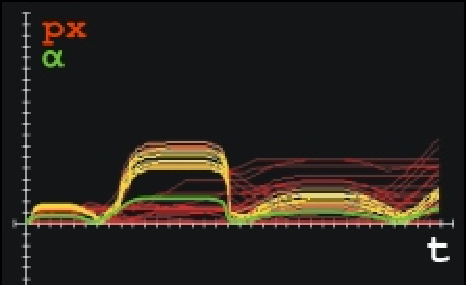
\includegraphics[width=3.5in]{imgs/method/correlation.ps}
		\caption[Trajectories correlating with the behaviour of the arm. ]{Trajectories correlating with the behaviour of the arm. All tracking trajectories of the qualified patches over time are red unless they do not match with the green motor joint trajectory and become yellow. On the left hand side we see an example with a positive result, on the right hand side obviously a negative.}
		\label{fig:corr}
	\end{center}
\end{figure}
%
In figure \ref{fig:corr} two different data sets are shown, where in the left set of trajectories there have been found patches matching to the self-actuated motion, on the other hand in the right hand non of the patches fit. $\rho_{corr}$ is adaptable, but experience show, later in \ref{results}, that under whatever conditions a range from 0.9 up to 0.97 are good thresholds. In figure \ref{fig:example} an experiment result is shown, where the patches $\in Q$ are displayed. The white circles (see image in the middle of figure \ref{fig:example}) denote the patches that are identified by the robot as patches following its motion.
%
%\begin{figure}[ht]
%	\begin{center}
%		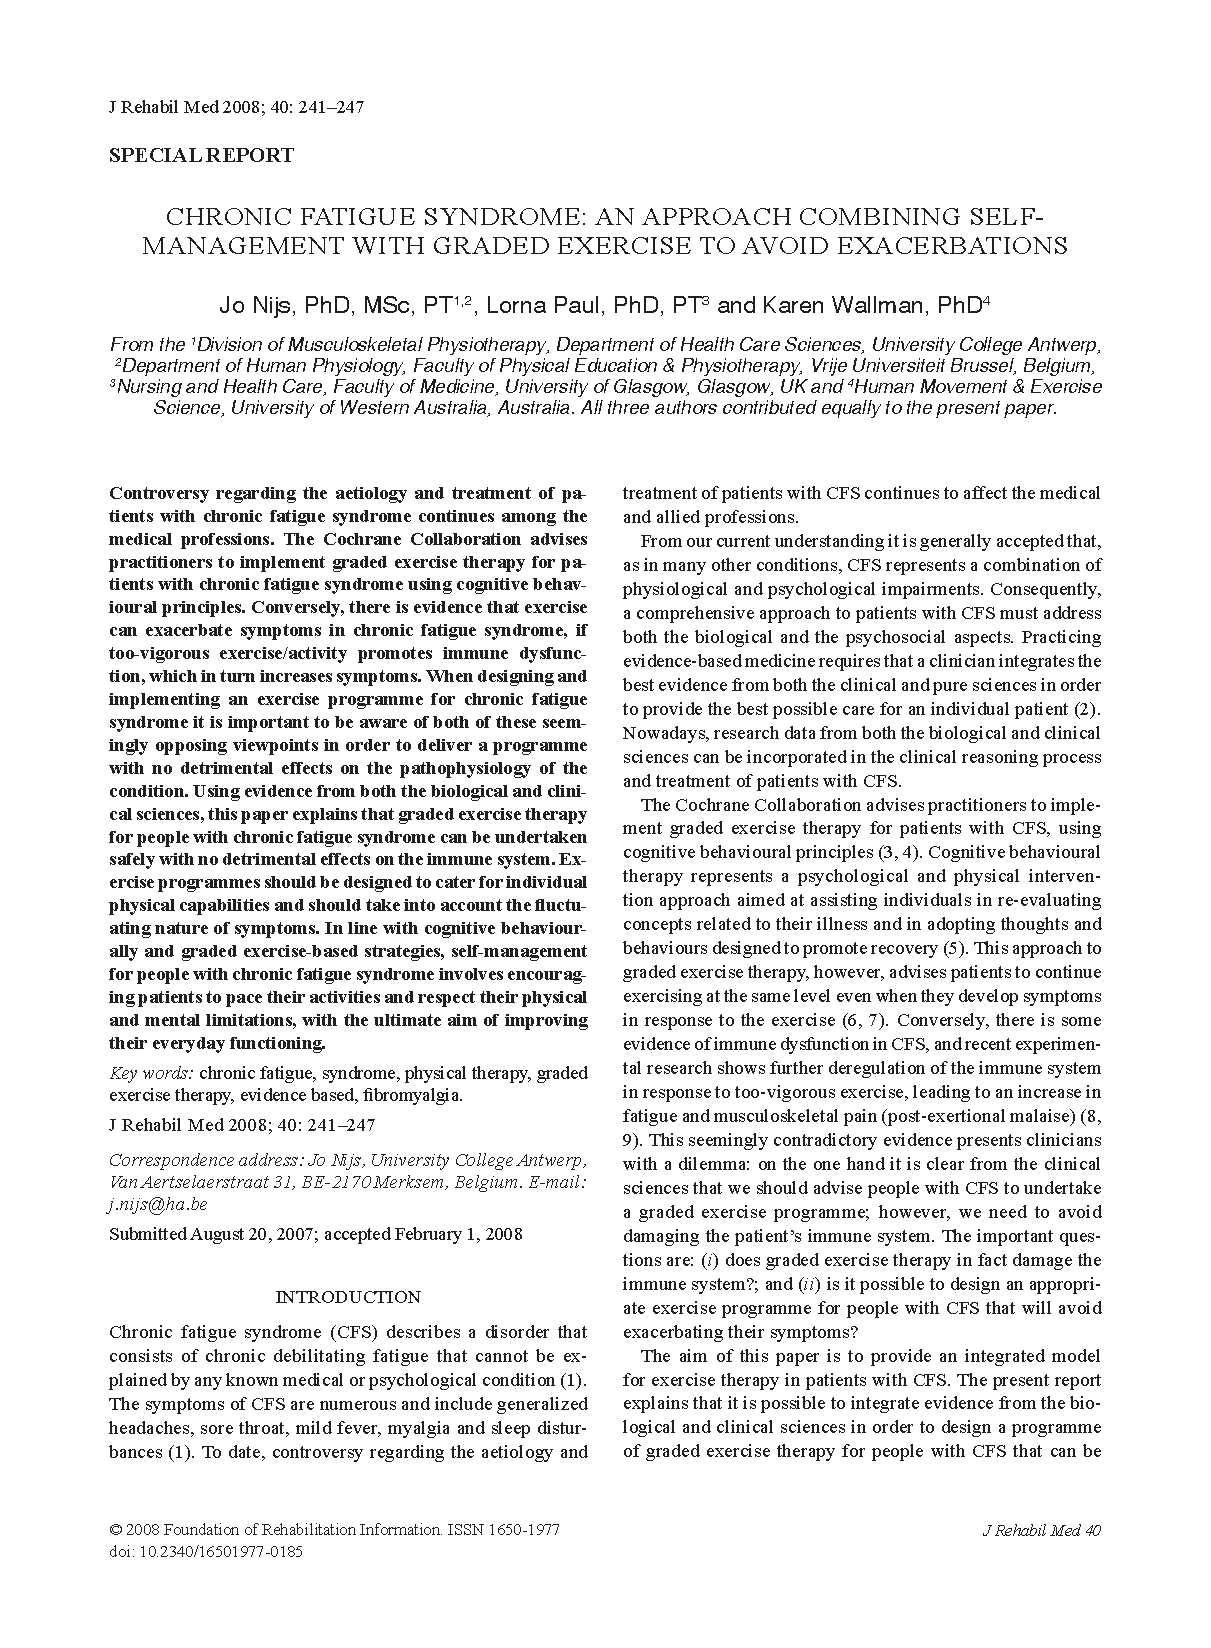
\includegraphics[width=.90\textwidth]{data/images/halo/example.jpg}
%		\caption[Hand localization of aperiodic arm motion. ]{Hand localization of aperiodic arm motion. In this example an aperiodic movement of the forearm generates the following result of the hand localization. On the most right (top), the selected region is elucidated by applying the convex hull over the resulting patch locations. Above we ``masked'' the ROI to explicitly show the reader the interesting region. }
%		\label{fig:example}
%	\end{center}
%\end{figure}
%
The patches correlating with the robot's actuated motion define a region of interest (ROI) where the hand is apparent. The convex hull around the selected patches is a way to mark the chosen ``hand'' area. Marking the ROI is as an intermediate step for the reader to understand how far we came with the localization, consult figure \ref{fig:roi}. The next step will segment the hand from this area.
%
%\begin{figure}[h]
%	\begin{center}
%		\includegraphics[width=.90\textwidth]{data/images/halo/roi.jpg}
%		\caption[Localized region of the hand. ]{Localized region of the hand. The region of interest is marked with the convex hull of the selected patches and denotes the location of the hand.  }
%		\label{fig:roi}
%	\end{center}
%\end{figure}
%
% -----------------------------------------------------------------------------------------------
%
%																						detection
%
\subsection{Detection (Segmentation)}\label{method:detection}
% -----------------------------------------------------------------------------------------------
Segmenting information means to extract or classify the one information, that we are interested in, from other ``useless'' information. In this particular case, the localization process returns a region of interest (ROI), see figure \ref{fig:example} on the outer right, denoted as the area where the hand, or parts of it, appear in the visive field. As we were not tracking (single) pixels from the hand but regions of ``equidirectional'' motion, we do not have the possibility to extract the hand. Still it is unclear how the hand looks like. The ROI contains the information about the hand, but unfortunately also parts of the environment.

The perfect way to extract all (moving) objects in front of a stationary scenery, is to subtract the \textit{known} background, seen in image \ref{fig:segmentation}. Explicitly we stress on the property: known background. But as we know a robot may act in different environments and e.g.\ moves its head, the background is not always the same and is rather a temporal constraint. The ROI defines a spatial window, which, observed over time, provides information for recovering the background. For recovering the background using the by-gone times A. Colombari et al.\ proposed a technique, described in section \ref{methods:bics}. Assuming that we can recover the background perfectly, an exact segmentation of the hand, or an excerpt of it limited by the ROI, is possible (see figure \ref{fig:perfsegm}). The visual model of the hand, given by the exact segmentation, provides the used information for later visually guide the robot's own hand in a reaching process.
%
\begin{figure}[h]
	\begin{center}
		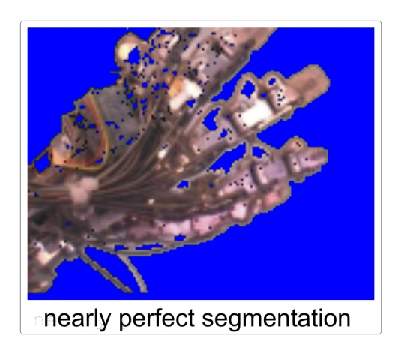
\includegraphics[width=3.5in]{imgs/method/perfsegm.ps}
	\end{center}
		\caption[Segmented hand. ]{Segmented hand. A nearly perfect segmentation of the hand extract gained by image $I_{t_{ready}+\tau_{tracking}}$ and the background gained with BICS, see page \pageref{methods:bics}.}
		\label{fig:perfsegm}
\end{figure}
%
\paragraph{Step 8: Segmentation:}
\label{halose:se8}
% 
At time $t_{ready}+ \tau_{tracking}$ we localized the hand. On the basis of the patches that were classified as part of the robot, we build a bounding box around the region of interest. Minimizing the area around the hand, enables to reduce the computing cost for retrieving the background and to increase the probability to extract only the hand and not other objects from the foreground. As above mentioned, we extract this bounding box from all the past images to recover the background. Once the background is computed, the foreground is a pixel-wise subtraction of the background from the region of interest. The values of the difference are binarized with a threshold, we used the same as in equation \ref{eq:bics:bindiff}. The binarization returns a mask, which is then applied on the image containing the extracted ROI and clearing the uninteresting (background) pixels. The procedure is illustrated in figure \ref{fig:segmentation}.
%
\begin{figure}[ht]
	\begin{center}
		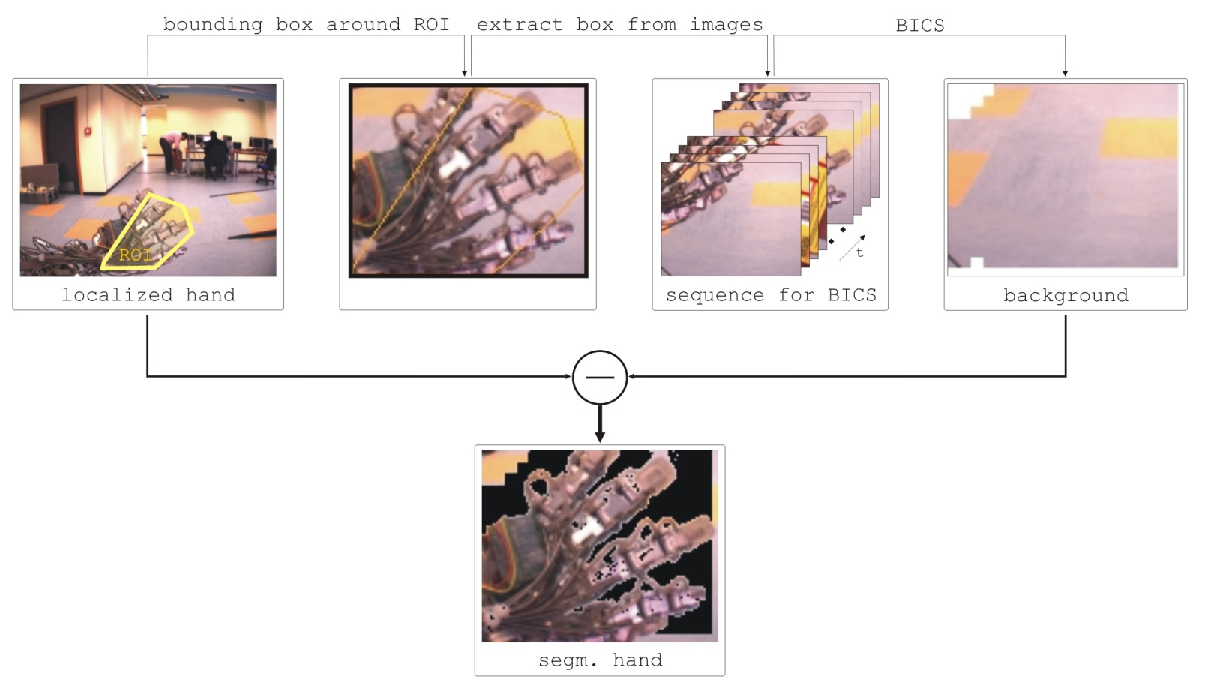
\includegraphics[width=3.5in]{imgs/method/segmentation.ps}
	\end{center}
		\caption[Detection procedure. ]{Detection procedure. At point in time $t_{ready}+ \tau_{tracking}$ we extract the bounding boxes from all images we the hand was localized. With the BICS algorithm the background is recovered. Finally the background is subtracted from the original image where the hand lies. Decision on the pixel differences is made on binarizing the values.}
		\label{fig:segmentation}
\end{figure}
%
\subsubsection{BICS}
\subsubsection{Problem}
